\documentclass[xcolor={dvipsnames}]{beamer}
\mode<presentation>
{
  \usetheme{Antibes}      % or try Darmstadt, Madrid, Warsaw, ...
  \usecolortheme{dolphin} % or try albatross, beaver, crane, ...
  \usefonttheme{professionalfonts}  % or try serif, structurebold, ...
  \setbeamertemplate{navigation symbols}{}
  \setbeamertemplate{caption}[numbered]
} 
\usepackage[utf8]{inputenc}
\usepackage[english]{babel}
\usepackage{multirow}
\usepackage{subfigure}
\usepackage{color}
\graphicspath{{/D:/fh/JI/latex/VE230 slides}}
\usepackage{amsmath}
\title[VE230 RC slides week 1]{VE230 RC slides Week 1}
\author{han.fang }
\date{\today}

\begin{document}

\begin{frame}
\titlepage
\end{frame}
\begin{frame}{Overview}
The first week only contains the content about the vectors. Thus, we would cover two things in this recitation class:
\newline
\begin{itemize}
	\item Vector review
	\item Coordinates
\end{itemize}
\end{frame}
\begin{frame}{Vectors}
dot product:
    $$
    \vec{A} \cdot \vec{B} = |\vec{A}||\vec{B}|cos\theta_{\vec{A}\vec{B}}
    $$
    \begin{itemize}
        \item Commutative: $\vec{A}\cdot\vec{B} = \vec{B}\cdot\vec{A}$
        \item Distributive: $\vec{A}\cdot(\vec{B} + \vec{C}) = \vec{A}\cdot\vec{B}+\vec{A}\cdot\vec{C}$
        \item Not associative: $\vec{A}\cdot(\vec{B}\cdot\vec{C}) \neq (\vec{A}\cdot\vec{B})\cdot\vec{C}$ 
        
        e.g. $(\vec{a_x}\cdot\vec{a_y})\cdot\vec{a_z} \neq \vec{a_x}\cdot(\vec{a_y}\cdot\vec{a_z})$
        \item For the three edges $A,B,C$ in a triangle, $C^2 = A^2 + B^2 - 2ABcos(\theta_{A,B})$
    \end{itemize}
\end{frame}
\begin{frame}{Vectors}
cross product:
    $$
    \vec{A}\times\vec{B} = \vec{a_n}||\vec{A}||\vec{B}|sin\theta_{\vec{A}\vec{B}}|
    $$
    \begin{itemize}
        \item The cross product is always perpendicular to both $\vec{A}, \vec{B}$, the direction follows right hand rule.
        \item Not Commutative: $\vec{A}\times\vec{B}\neq\vec{B}\times\vec{A}$ (have opposite directions).
        \item Distributive: $\vec{A}\times(\vec{B}+\vec{C}) = \vec{A}\times\vec{B} + \vec{A}\times\vec{C}$
        \item Not associative: $\vec{A}\times(\vec{B}\times\vec{C}) \neq (\vec{A}\times\vec{B})\times\vec{C}$
        
        e.g. $\vec{a_x}\times(\vec{a_x}\times\vec{a_y}) = \vec{a_x}\times\vec{a_z} = -\vec{a_y}$, 

        $(\vec{a_x}\times\vec{a_x})\times\vec{a_y} = 0\neq -\vec{a_y}$
    \end{itemize}
\end{frame}
\begin{frame}{Vectors}
\begin{block}{Some useful rules:}
\begin{itemize}
	\item $\vec{A}\cdot(\vec{B}\times\vec{C}) = \vec{B}\cdot(\vec{C}\times\vec{A}) = \vec{C}\cdot(\vec{A}\times\vec{B}) = Volume$
    \item BAC-CAB:
        $\vec{A}\times(\vec{B}\times\vec{C}) = \vec{B}(\vec{A}\cdot\vec{C}) - \vec{C}(\vec{A}\cdot\vec{B})$
\end{itemize}
\end{block}


\end{frame}
\begin{frame}{Review Exercises}
P.2-1 Given three vectors $\vec{A},\vec{B}$ and $\vec{C}$ as follows,
    
    $\vec{A}=\vec{a_x}+\vec{a_y}2-\vec{a_z}3$,

    $\vec{B}=-\vec{a_y}4+\vec{a_z}$,

    $\vec{C}=\vec{a_x}5-\vec{a_z}2$,

    find
    \begin{itemize}
        \item[a)] $\vec{a_A}$: note $a_A$ represents the unit vector of $\vec{A}$.
        \break
        \pause
        We can obtain that
        $$a_{A}=\frac{1}{\sqrt{1^2+2^2+3^2}}\vec{A}.$$
    \end{itemize}

\end{frame}
\begin{frame}{Review Exercises}
P.2-1 Given three vectors $\vec{A},\vec{B}$ and $\vec{C}$ as follows,
    
    $\vec{A}=\vec{a_x}+\vec{a_y}2-\vec{a_z}3$,

    $\vec{B}=-\vec{a_y}4+\vec{a_z}$,

    $\vec{C}=\vec{a_x}5-\vec{a_z}2$,

    find
    \begin{itemize}
        \item[b)] $b_{c}$:the component of $\vec{A}$ in the direction of $\vec{C}$
        \break
        \pause
        We can obtain that
        $$b_{c}=\frac{\vec{A}\cdot\vec{C}}{|\vec{C}|}=\frac{11}{\sqrt{29}}$$
    \end{itemize}
\end{frame}
\begin{frame}{Review Exercises}
P.2-1 Given three vectors $\vec{A},\vec{B}$ and $\vec{C}$ as follows,
    
    $\vec{A}=\vec{a_x}+\vec{a_y}2-\vec{a_z}3$,

    $\vec{B}=-\vec{a_y}4+\vec{a_z}$,

    $\vec{C}=\vec{a_x}5-\vec{a_z}2$,

    find
    \begin{itemize}
        \item[c)] $\vec{A}\times\vec{C}$ (1. use properties; 2. calculate by matrix)
        \break
        \pause
        \begin{itemize}
        	\item $\vec{a_x}\times\vec{a_x}=0,\vec{a_x}\times\vec{a_y}=\vec{a_z},...$
        	\item direct product by matrix
        \end{itemize}
        Answer is
        $$\vec{A}\times\vec{C}=-4\vec{a_x}-13\vec{a_y}+10\vec{a_z}.$$
    \end{itemize}
\end{frame}
\begin{frame}{Review Exercises}
P.2-1 Given three vectors $\vec{A},\vec{B}$ and $\vec{C}$ as follows,
    
    $\vec{A}=\vec{a_x}+\vec{a_y}2-\vec{a_z}3$,

    $\vec{B}=-\vec{a_y}4+\vec{a_z}$,

    $\vec{C}=\vec{a_x}5-\vec{a_z}2$,

    find
    \begin{itemize}
        \item[d)] prove $\vec{A}\cdot(\vec{B}\times\vec{C})=(\vec{A}\times\vec{B})\cdot\vec{C}$
    \end{itemize}
\end{frame}
\begin{frame}{Review Exercises}
P.2-1 Given three vectors $\vec{A},\vec{B}$ and $\vec{C}$ as follows,
    
    $\vec{A}=\vec{a_x}+\vec{a_y}2-\vec{a_z}3$,

    $\vec{B}=-\vec{a_y}4+\vec{a_z}$,

    $\vec{C}=\vec{a_x}5-\vec{a_z}2$,

    find
    \begin{itemize}
        \item[e)] $(\vec{A}\times\vec{B})\times\vec{C}$ and $\vec{A}\times(\vec{B}\times\vec{C})$ (convert the form to the standard BAC-CAB)
    \end{itemize}
    \pause
    \break
    \begin{itemize}
    	\item $(\vec{A}\times\vec{B})\times\vec{C}=-\vec{C}\times(\vec{A}\times\vec{B})$
    	\item $\vec{A}\times(\vec{B}\times\vec{C}) = \vec{B}(\vec{A}\cdot\vec{C}) - \vec{C}(\vec{A}\cdot\vec{B})$
    \end{itemize}
\end{frame}
\begin{frame}{Review Exercises}
\begin{block}{P.2-2}
Given 
    $$\vec{A}=\vec{a_x}-\vec{a_y}2+\vec{a_x}3$$, $$\vec{B}=\vec{a_x}+\vec{a_y}-\vec{a_z}2$$, find the expression for a unit vector $\vec{C}$ that is perpendicular to both $\vec{A}$ and $\vec{B}$.
\end{block}
\pause
$$\vec{C}=\frac{\vec{A}\times\vec{B}}{|\vec{A}\times\vec{B}|}$$
\end{frame}
\begin{frame}{Review Exercises}
\begin{block}{P.2-4}
Show that, if $\vec{A}\cdot\vec{B} = \vec{A}\cdot\vec{C}$ and $\vec{A}\times\vec{B} = \vec{A}\times\vec{C}$, where $\vec{A}$ is not a null vector, then $\vec{B}=\vec{C}$.
\end{block}
\pause
\begin{itemize}
	\item $\vec{A}\cdot\vec{B} = \vec{A}\cdot\vec{C}\rightarrow \vec{A}\perp (\vec{B}-\vec{C})$
	\item $\vec{A}\times\vec{B} = \vec{A}\times\vec{C}\rightarrow \vec{A}\parallel (\vec{B}-\vec{C})$
\end{itemize}
Since A is not null, it is obvious that $\vec{B}-\vec{C}=\vec{0}$
\end{frame}
\begin{frame}{Coordinates}
Three basis $(u_1, u_2, u_3)$: number of linearly independent basis = dimension of the space. For the three types of coordinates we discuss, $u_i$ is orthogonal to each other.

For arbitrary vector $\vec{A}$:

$$\vec{A} = \vec{a_{u1}}A_{u1} + \vec{a_{u2}}A_{u2} + \vec{a_{u3}}A_{u3}$$,

Norm of $\vec{A}$:
$$|\vec{A}| = \sqrt{A_{u1}^2 + A_{u2}^2 + A_{u3}^2}$$

For a differential length $dl$, 

$$dl = \vec{a_{u1}}(h_1du_1) + \vec{a_{u2}}(h_2du_2) + \vec{a_{u3}}(h_3du_3)$$ $h_i$ is called metric coefficient.

\end{frame}
\begin{frame}{Coordinates}
differential volume:

$$dv = h_1h_2h_3du_1du_2du_3$$

differential area vector with a direction normal to the surface,

$$d\vec{s} = \vec{a_n}ds$$

differential area $ds_1$ normal to the unit vector $\vec{a_{u1}}$.
\end{frame}
\begin{frame}{Cartesian Coordinates}
\begin{itemize}
    \item $$(u_1, u_2, u_3) = (x, y, z)$$
    \item Right hand rule:
    $$
    \vec{a_x}\times\vec{a_y} = \vec{a_z}
    $$
    \item 
    $$
    \vec{A} = \vec{a_x}A_x + \vec{a_y}A_y + \vec{a_z}A_z
    $$,
    where $\vec{a_i}$ is the basis for i-axis.
    

\end{itemize}
\end{frame}
\begin{frame}{Cartesian Coordinates}
\begin{itemize}
	\item dot product and cross product:
	$$\vec{a_x}\cdot\vec{a_x}=1,\vec{a_x}\times\vec{a_y}=\vec{a_z}.$$
    \item differential length:
    \begin{equation}\label{Eq: cartesian-differential-length}
        d\vec{l} = \vec{a_x}dx + \vec{a_y}dy + \vec{a_z}dz
    \end{equation}
    \item differential area:

    $$
    ds_x = dydz
    $$,
    as $h_1 = h_2 = h_3 = 1$,

    ($ds_x$ is the surface perpendicular to the x-axis, the forms for other surfaces follow the same pattern).
    \item differential volume:

    $$
    dv=dxdydz
    $$
\end{itemize}
\end{frame}
\begin{frame}{Cylindrical Coordinate}
\begin{itemize}
    \item $$(u_1, u_2, u_3) = (r, \phi, z)$$
    Claim: as $a_r$ can change its direction in the x-y plane, vectors in x-y plane could be represented simply by $\vec{a_r}$. Thus, all vectors in cylindrical coordinate could be represented by $\vec{a_r}$ and $\vec{a_z}$.

    \item Right hand rule: 
    $$\vec{a_r}\times\vec{a_\phi}=\vec{a_z}$$
    \item $$\vec{A} = \vec{a_r}Ar + \vec{a_\phi}A_\phi + \vec{a_z}A_z$$
    \item differential length:
    \begin{equation}\label{Eq: cylindrical-differential-length}
        d\vec{l} = \vec{a_r}dr + \vec{a_\phi}rd\phi + \vec{a_z}dz
    \end{equation},
    as $h_1 = 1, h_2 = r, h_3 = 1$
\end{itemize}
\end{frame}
\begin{frame}{Cylindrical Coordinate}
\begin{itemize}
    \item differential area: 
    $$
    ds_r = rd\phi dz
    $$

    \item differential volume:
    $$
    dv = rdrd\phi dz
    $$
    \item From cylindrical coordinate to Cartesian coordinate: represent $A_x$ by the quantities in cylindrical coordinate.The same applies to $A_y$.

\end{itemize}
\end{frame}
\begin{frame}{Cylindrical Coordinate}
Conversion of quantities between Cartesian coordinate and Cylindrical coordinate:
    \begin{enumerate}
   
        \item
        $$
        \begin{cases}
            x = rcos\phi\\
            y = rsin\phi\\
            z = z
        \end{cases}
        $$
        \item
        $$
        \begin{cases}
            r= \sqrt{x^2 + y^2}\\
            \phi = arctan \frac{y}{x}\\
            z = z
        \end{cases}
        $$
    \end{enumerate}
You can try to write the conversion between $dx,dy,dz$ and $dr,d\phi,dz$.
\end{frame}
\begin{frame}{Cylindrical Coordinate}
The conversion between $dx,dy,dz$ and $dr,d\phi,dz$:
\begin{figure}
	\centering
	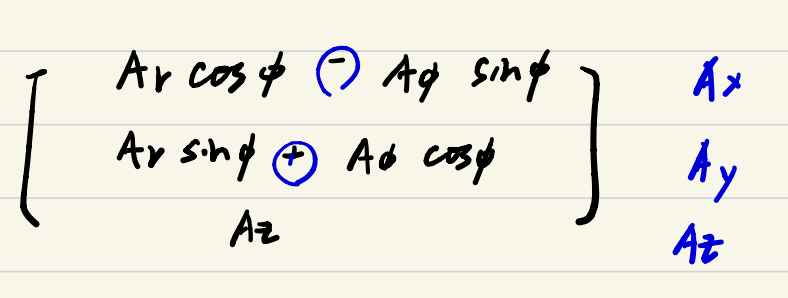
\includegraphics[width=0.7\linewidth]{1.png}
\end{figure}
\end{frame}
\begin{frame}{Spherical Coordinate}
\begin{itemize}
    \item Figure for Spherical Coordinate. Notice the position of $\phi, \theta$.
    \item
    $$
    (u_1, u_2, u_3) = (R, \theta, \phi)
    $$
    \item Right hand rule: 
    $$
    \vec{a_R} \times \vec{\theta} = \vec{\phi}
    $$
    \item $$
    \vec{A} = \vec{a_R}A_R + \vec{a_\theta}A_\theta + \vec{a_\phi}A_\phi
    $$
    \item differential length:
    \begin{equation}\label{Eq: spherical-differential-length}
        d\vec{l} = \vec{a_R}dR + \vec{a_\theta}Rd\theta + \vec{a_\phi}Rsin\theta d\phi
    \end{equation}, as $h_1 = 1, h_2 = R, h_3 = Rsin\theta$.
    \item differential area:
    $$
    ds_R = R^2sin\theta d\theta d\phi
    $$
\end{itemize}
\end{frame}
\begin{frame}{Spherical Coordinate}
\begin{itemize}
    \item differential volume: 
    $$
    dv = R^2 sin\theta dR d\theta d\phi
    $$
    \item conversion of quantities between Cartesian coordinate and Spherical coordinate:
    \begin{enumerate}
        \item
        $$
        \begin{cases}
            x = Rsin\theta cos\phi\\
            y = Rsin\theta sin\phi\\
            z = Rcos\theta
        \end{cases}
        $$
        \item
        $$
        \begin{cases}
            R=\sqrt{x^2+y^2+z^2}\\
            \theta = arctan\frac{\sqrt{x^2+y^2}}{z}\\
            \phi = arctan\frac{y}{x}
        \end{cases}
        $$
    \end{enumerate}
    \item From Spherical coordinate to Cartesian coordinate: represent $A_x$ by the quantities in Spherical coordinate; write the formula in the form of matrix. (Similar to cylindrical coordinate).
\end{itemize}
\end{frame}

\begin{frame}{Review Exercises}
\begin{block}{P.2-17}
 A field is expressed in spherical coordinates by $\vec{E} = \vec{a_R}(25/R^2)$.
\begin{itemize}
    \item [b)] Find the angle that $\vec{E}$ makes with the vector $\vec{B} = \vec{a_x}2 - \vec{a_y}2 + \vec{a_z}$ at point $P(-3, 4, -5)$.
\end{itemize}
\end{block}
\pause
\begin{block}{Answer}
$$\cos(\theta)=\frac{\vec{E}\cdot\vec{B}}{|\vec{E}|\cdot|\vec{B}|}.$$
\end{block}
\end{frame}
\begin{frame}{Review Exercises}
Express the base vectors $\vec{a_x},\vec{a_y}, \vec{a_z}$ of a Cartesian coordinate in spherical coordinate system.
\pause
\begin{figure}[H]
	\centering
	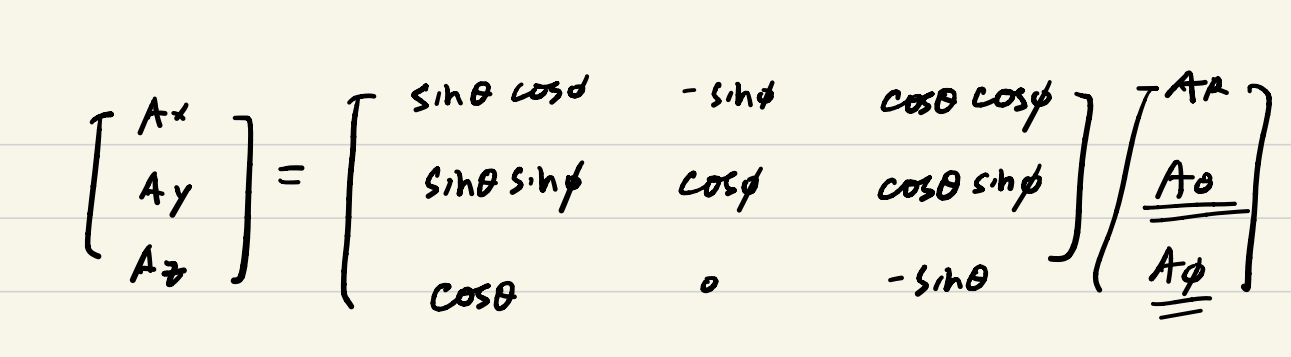
\includegraphics[width=0.7\linewidth]{2.png}
\end{figure}
\end{frame}
\begin{frame}{Review Exercises}
\begin{block}{P.2-19}
Determine the values of the following products of base vectors.
\begin{itemize}
    \item [a)] $\vec{a_x}\cdot\vec{a_\phi}$
    \item [c)] $\vec{a_r}\times\vec{a_x}$ 
\end{itemize}
\end{block}
\pause
\begin{block}{Answer}
\begin{itemize}
    \item [a)] $\vec{a_x}\cdot\vec{a_\phi}=\cos (\frac{\pi}{2}+\phi)$
    \item [c)] $\vec{a_r}\times\vec{a_x}=-\vec{a_z}\sin (\phi)$ 
\end{itemize}
\end{block}
\end{frame}
\begin{frame}{Further plans}
In the future RC classes, I will review some problems in the homework. You can turn in your assignment directly in my RC classes. Though the assignment might not be graded in details and not counted into the final grade, we still hope you can come to the RC and submit your assignments during the RC, which will not take so much time. The assignments will give you a basic review about the course material, which will be so beneficial for your exam and quiz. 

\end{frame}



\end{document}
